\chapter{Week 02} % The Chamber of Pythonistas

\section{PyCon}
    
    % \begin{wrapfigure}{R}{0.5\textwidth}
    %     \centering
    %     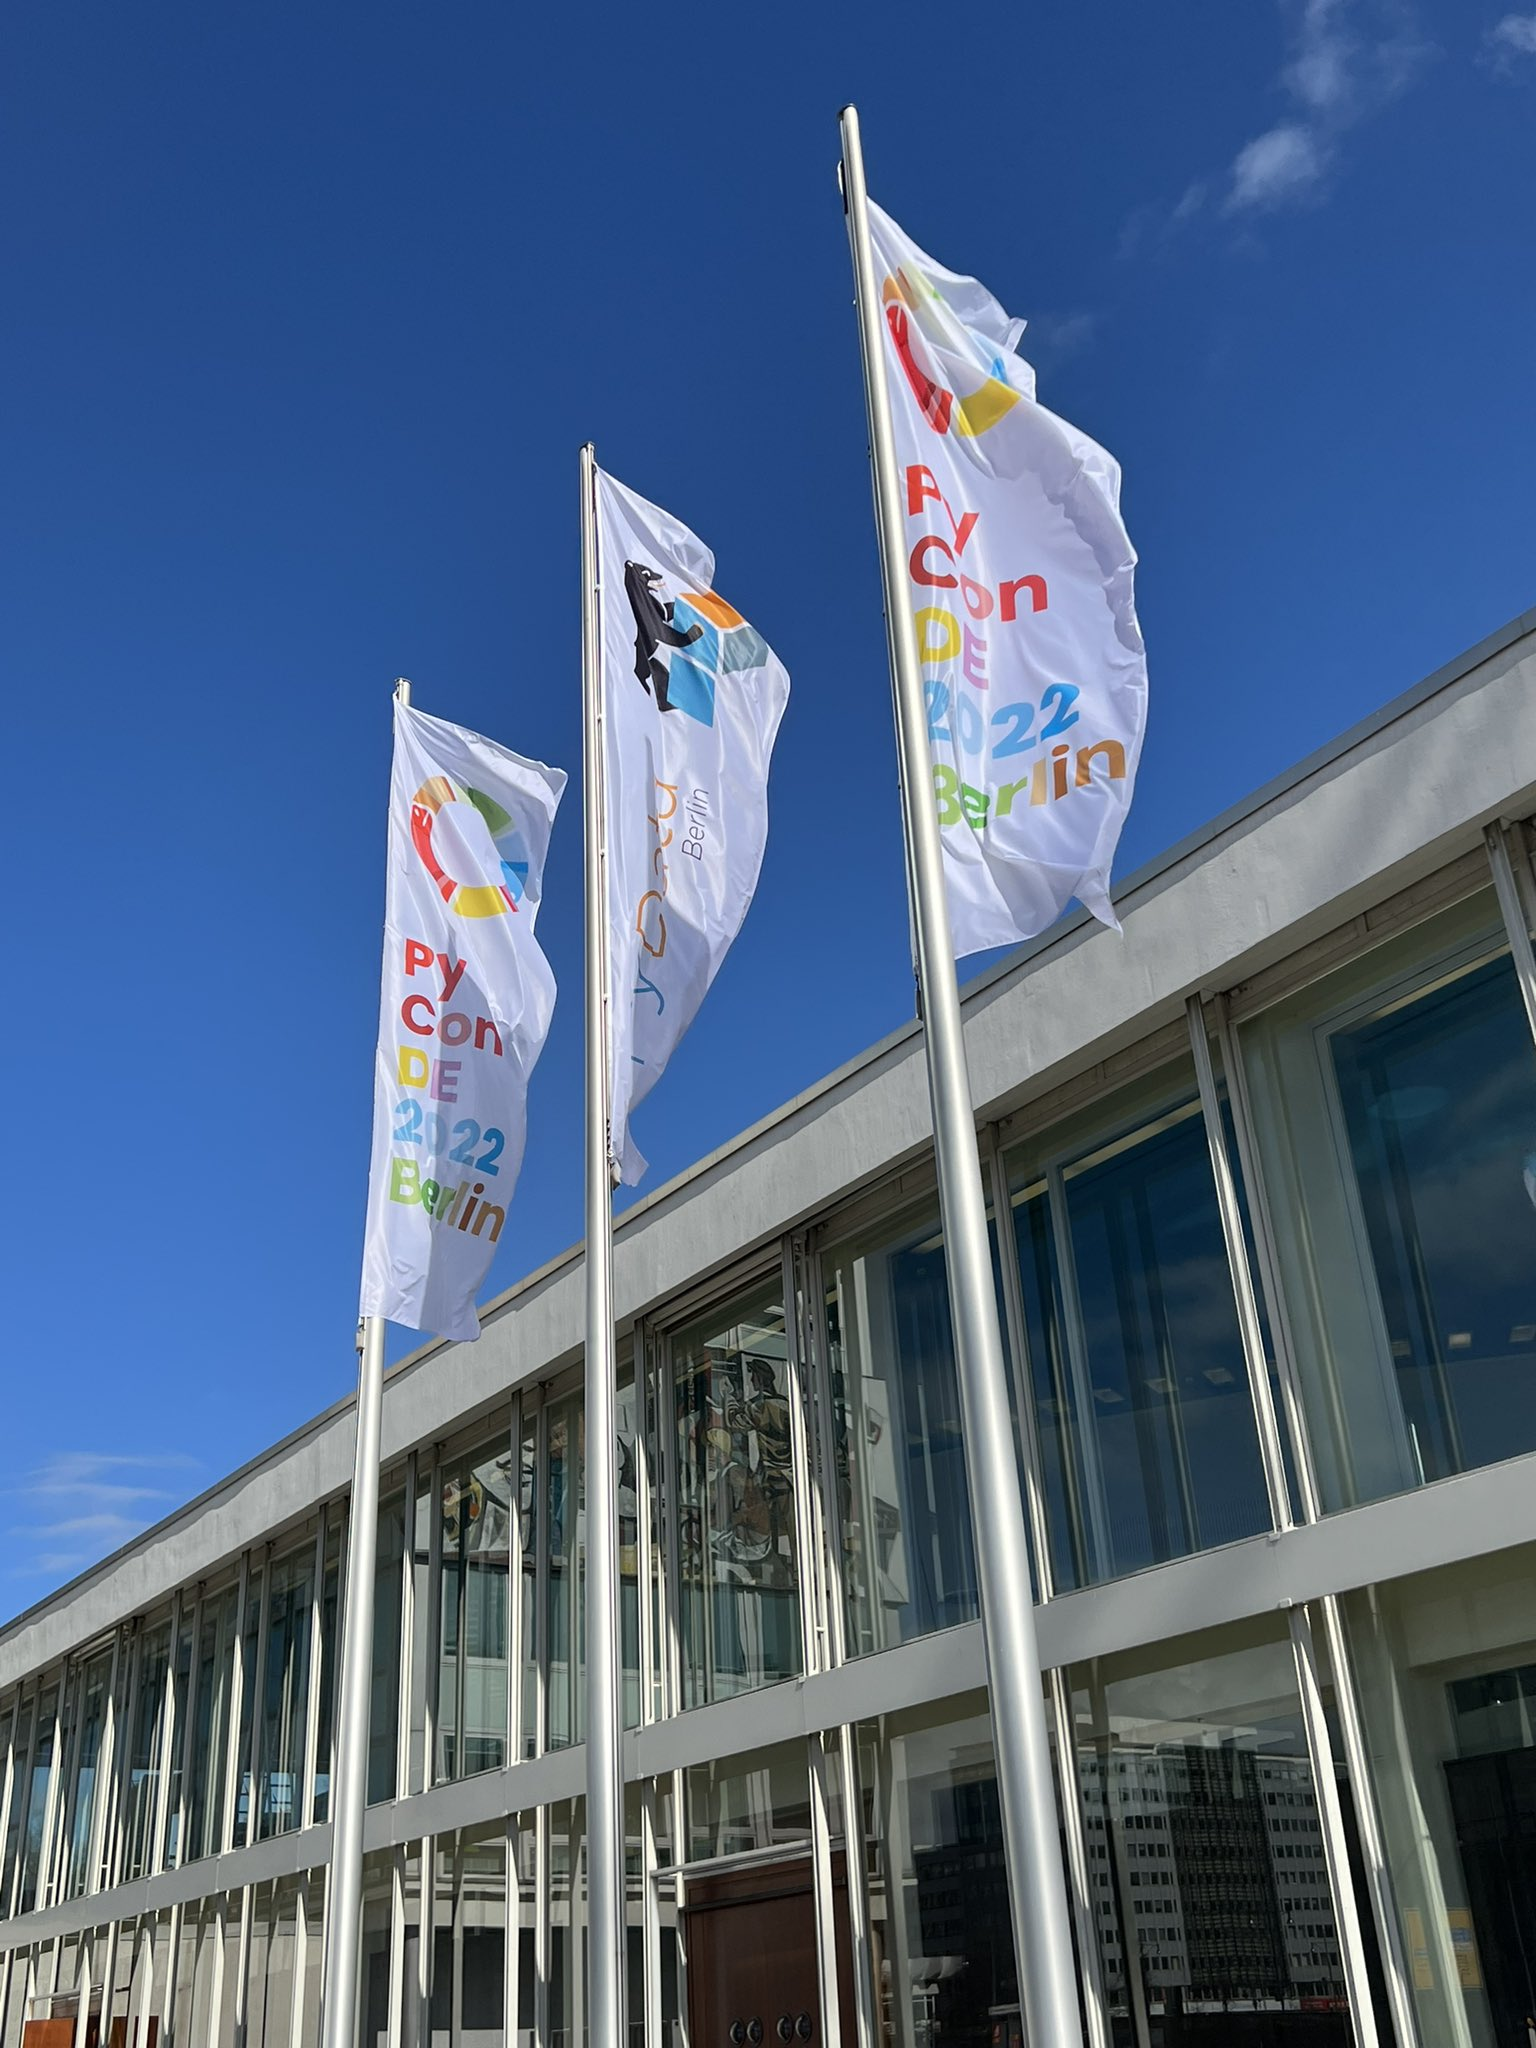
\includegraphics[width=0.45\textwidth]{Images/02_pyCon.jpeg}
    %     \caption{Photograph of BCC by \href{https://twitter.com/__pamaron__}{Ernesto Arbitrio}}
    %     \label{fig:pycon}
    % \end{wrapfigure}
    
    This week mainly consisted of attending PyCon DE and PyData Berlin. This was a three-day event held at the Berlin Congress Center (Figure \ref{fig:pycon}). During the conference, there were several talks conducted by Python experts. The following are a few highlights from the talks attended:
    \begin{itemize}
        \item \href{https://player.vimeo.com/video/698423690}{\textit{Trojan Source Malware}} by Cheuk Ting Ho $\rightarrow$ It is a bad practice to blindly copy code from the internet because there could be hidden ASCII characters which may result in undesirable program behavior.
        \item \textit{Your Data, Your Insights} by Paula Gonzalez $\rightarrow$ Developing projects to visualize one's own personal data is another way to rekindle the joy for data science.
        \item \textit{Can You Read This?} by Asya Frumkin $\rightarrow$ To aid people with visual impairments, it is the duty of developers to consider text readability on uniform and non-uniform backgrounds.
        \item \textit{The Magic of Python Objects} by Coen de Groot $\rightarrow$ Magic or Dunder methods can be overridden in a custom class to create overloaded behaviors. 
        \item \href{https://blog.jupyter.org/jupyterlite-jupyter-%EF%B8%8F-webassembly-%EF%B8%8F-python-f6e2e41ab3fa}{\textit{JupyterLite}} by Jeremy Tuloup $\rightarrow$ JupyterLite is another version of JupyterLab which runs entirely on a web browser without the need to install anything. 
    \end{itemize} 
    
    \begin{figure}[hb]
        \centering
        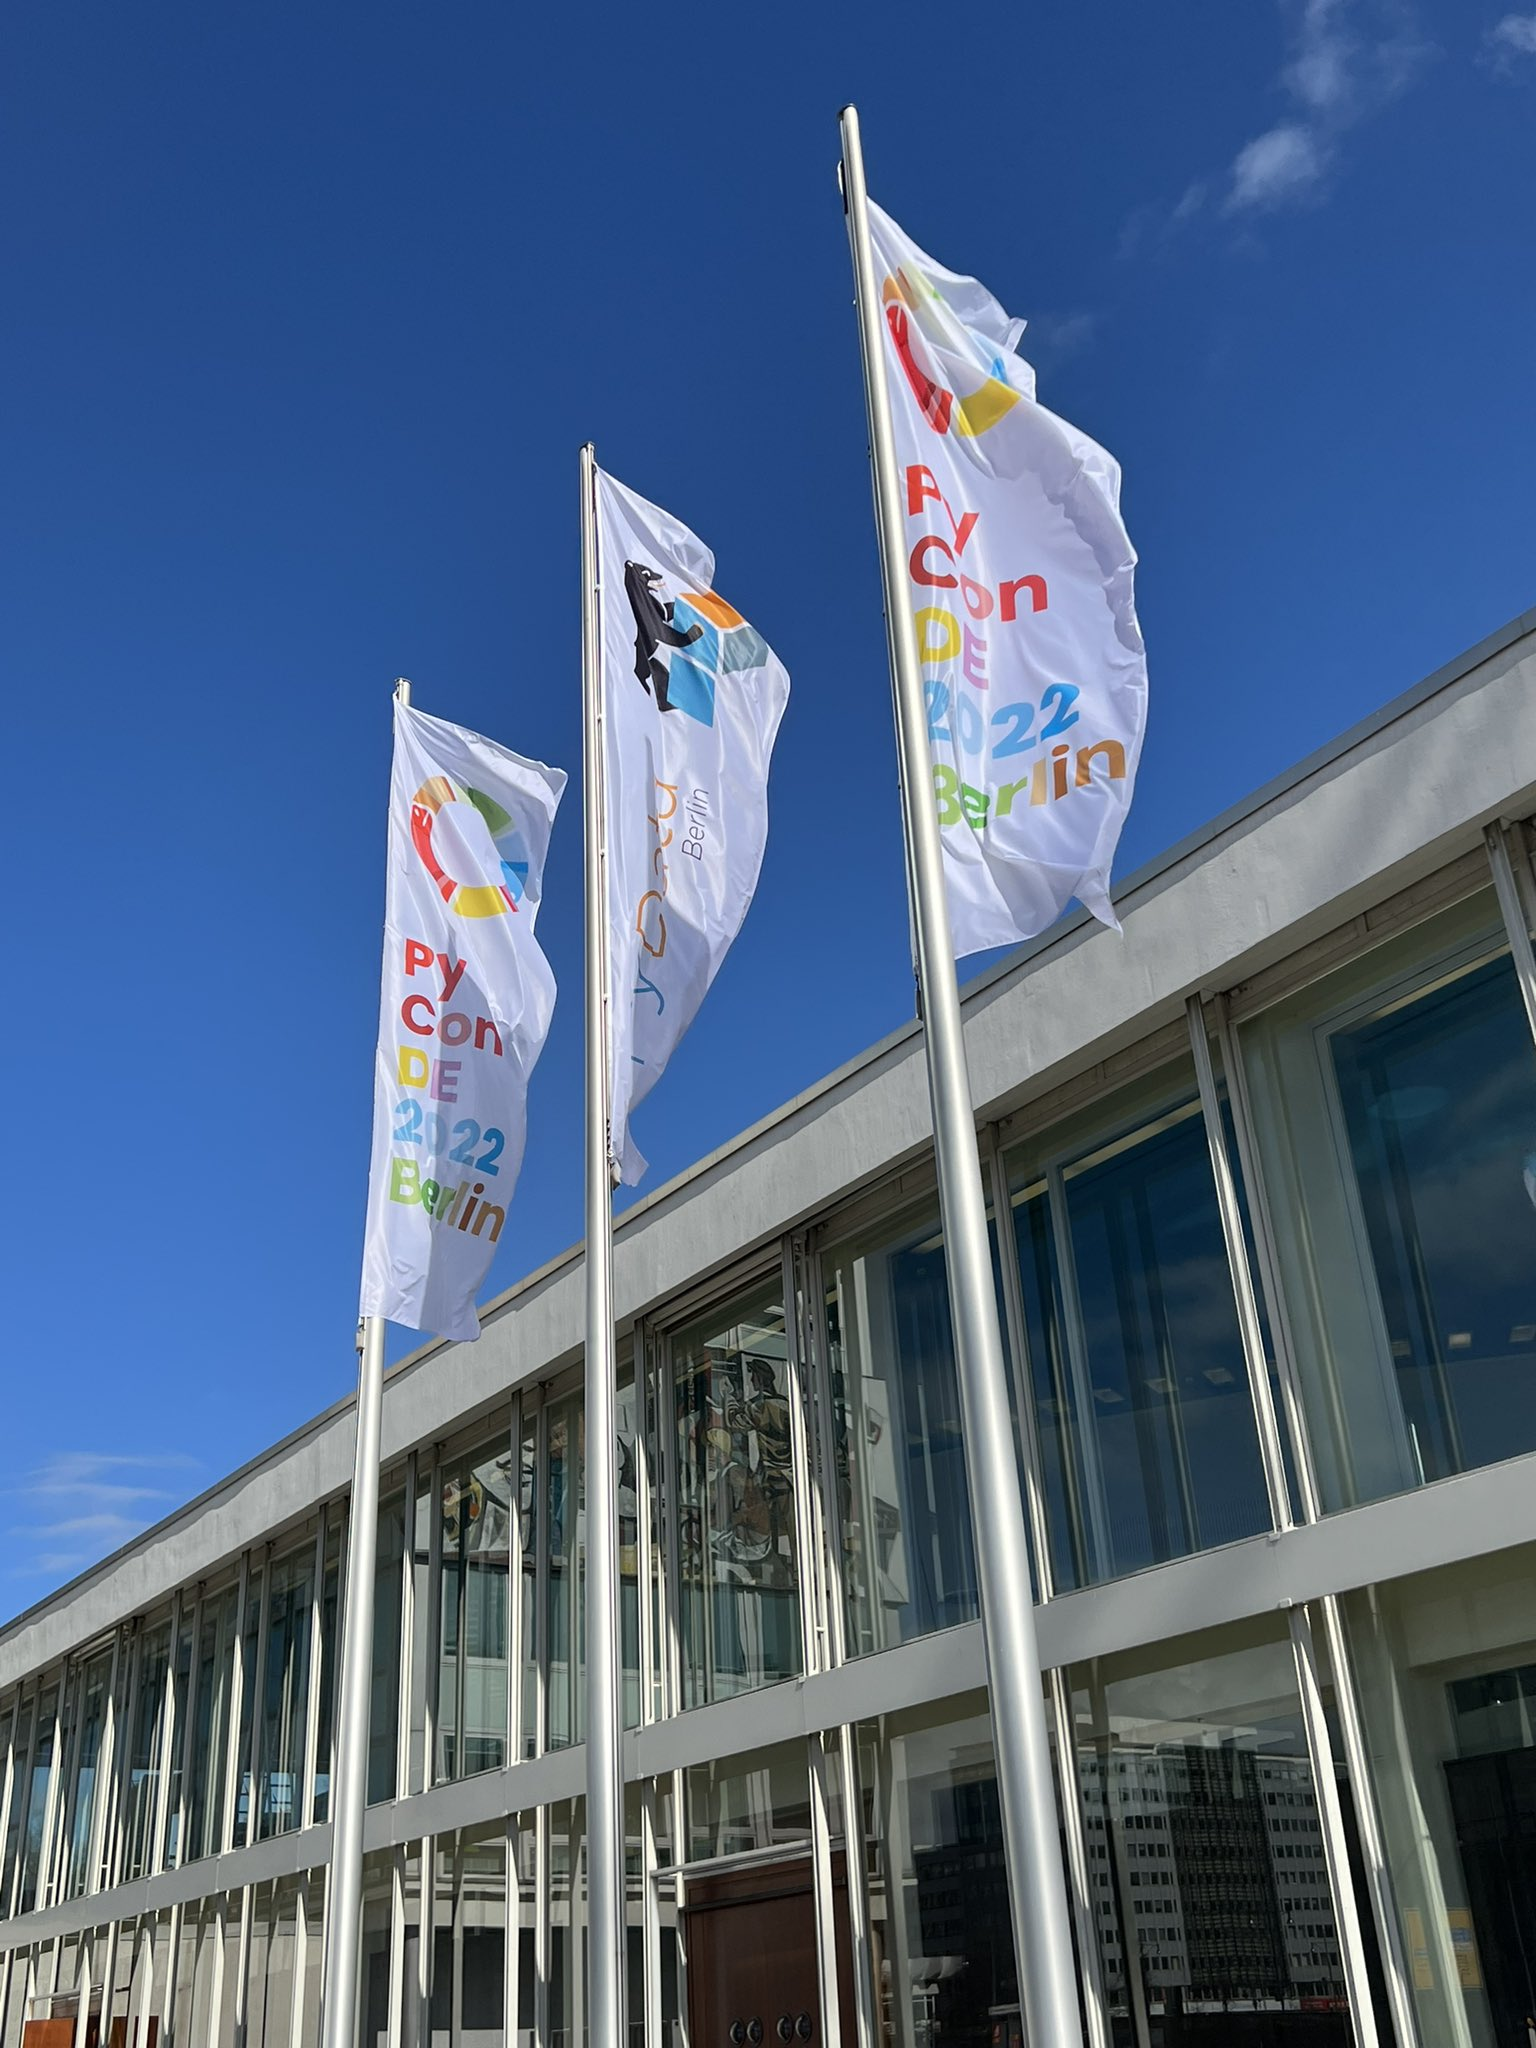
\includegraphics[width=0.45\linewidth]{Images/02_pyCon.jpeg}
        \caption{Photograph of BCC by \href{https://twitter.com/__pamaron__}{Ernesto Arbitrio}}
        \label{fig:pycon}
    \end{figure}
    
    % \begin{itemize}
    %     \item \textbf{What I learned from monitoring more than 30 Machine Learning Use Cases} by Lina Weichbrodt
    %     \item \textbf{Creating 3D Maps using Python} by Martin Christen
    %     \item \textbf{Trojan Source Malware - Can we trust open-souce anymore?} by Cheuk Ting Ho
    %     \item \textbf{conda-forge: supporting the growth of the volunteer-driven, community-based packaging project} by Wolf Vollprecht, Jannis Leidel and Jaime Rodríguez-Guerra
    %     \item \textbf{JupyterLite: Jupyter WebAssembly Python} by Jeremy Tuloup
    %     \item \textbf{Slack bots 101: An introduction into slack bot-based workflow automation} by Jordi Smit
    %     \item \textbf{Your data, your insights: creating personal data projects to (re-)own the data you share} by Paula Gonzalez Avalos
    %     \item \textbf{Python 3.11 in the Web Browser - A Journey} by Christian Heimes
    %     \item \textbf{Fast native data structures: C/C++ from Python} by Stefan Behnel
    %     \item \textbf{Squirrel - Efficient Data Loading for Large-Scale Deep Learning} by Dr. Thomas Wollmann
    %     \item \textbf{Can You Read This? Or: how I Improved text readability on the Web for the Visually Impaired} by Asya Frumkin
    %     \item \textbf{The Magic of Python Objects} by Coen de Groot
    %     \item \textbf{How to Find Your Way Through a Million Lines of Code} by Jürgen Gmach
    %     \item \textbf{There Are Python 2 Relics in Your Code} by Miroslav Šedivý
    % \end{itemize}
    

    \section{Turtlesim II}
    
        To continue the work from last week, a \texttt{TurtleWidget} class was created. This class contains the following methods:
        \begin{itemize}
            \item \texttt{randomize} $\rightarrow$ this method selects a random turtle image with the exception of the turtle named \textit{palette} because this image does not appear to be a turtle.
            \item \texttt{spawn} $\rightarrow$ this method spawns a turtle in the middle of the canvas if no specified spawning pose is given.
            \item \texttt{move\_to\_pose} $\rightarrow$ this method draws the turtle at the new pose given and generates a line from the old position to the new position.
            \item \texttt{draw\_turtle} $\rightarrow$ this method transforms the canvas to be able to draw the turtle at the specified position and orientation.
        \end{itemize}
        
        Initially, some flickering issues had been observed while performing the animation, this had been resolved by using two canvas layers dedicated to the turtle so that there could always be a turtle visible on the overall canvas. However, the flickering was no longer observed after creating the class, thus, the multi-canvas was reduced to only three layers: background, path, and turtle.
        
        The generated linear path appears to be working correctly as is illustrated in Figure \ref{fig:linePath}. However, if the turtle takes a sharp turn, the intersection of the lines is not as smooth as it could be. This could potentially be resolved by dropping a circular marker at every turn but it could also slow down the performance.
        
        Lastly, a spiral path publisher was created to generate the path seen in Figure \ref{fig:spiralPath}. This publisher follows the Archimedean spiral equations to traverse five loops from the center of the canvas.
        
        \begin{figure}[hb]
            \centering
            \begin{subfigure}{.55\textwidth}
                \centering
                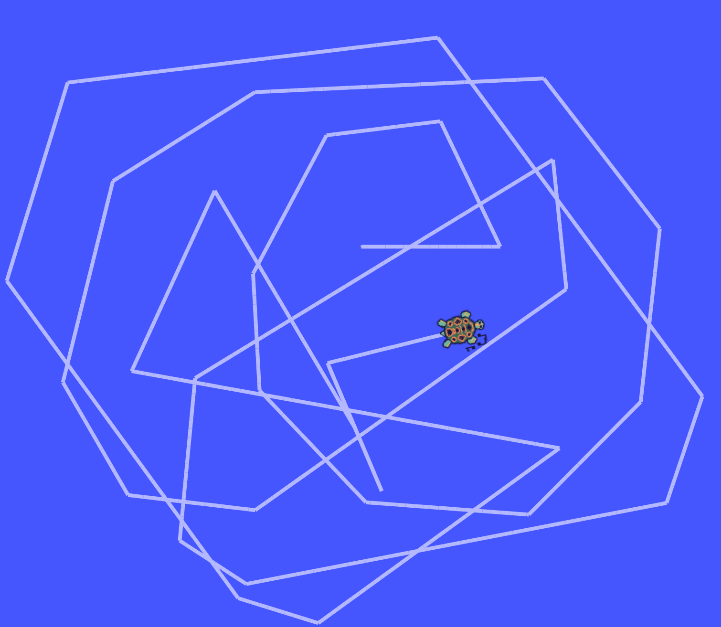
\includegraphics[height=6cm]{Images/02_linePath.png}
                \caption{Linear path created from saving previous position.}
                \label{fig:linePath}
            \end{subfigure}%
            \begin{subfigure}{.45\textwidth}
                \centering
                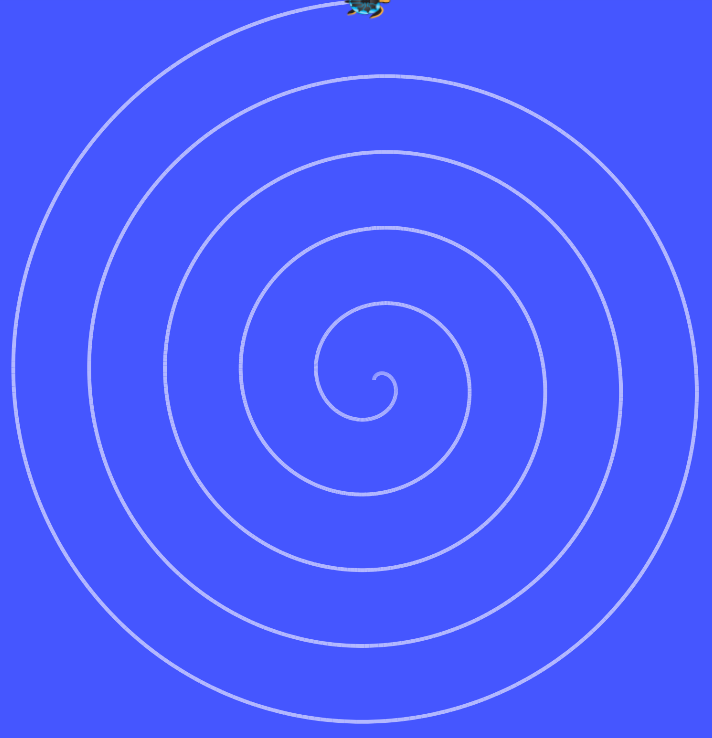
\includegraphics[height=6cm]{Images/02_turtleSpiral.png}
                \caption{Path drawn by the spiral publisher.}
                \label{fig:spiralPath}
            \end{subfigure}
            \caption{Turtle paths}
            \label{fig:turtlePaths}
        \end{figure}
    
    
    
    \section{Future Work}
    
        For the next steps, it would be useful to be able to call a spawn service to display new turtles on the canvas. This could be implemented by adding an additional canvas layer for every new turtle, or by simply storing the information for each turtle separately and keeping all the turtle images on the same layer.